\section{Gestion des Notifications Téléphoniques : Aerogear}

Les notifications ont une place importante dans l'application téléphonique Dynamease. Ce sont grâce à celles-ci que les informations sur l'appelant sont récupérées par l'appareil. 

\subsection{Fonctionnement des notifications Push}

Une notification est un message envoyé à un smartphone. Ce message à la possibilité de réveiller le smartphone et d'afficher une information. L'envoi d'une notification nécessite une plateforme. Pour envoyer une notification à un appareil Android la plateforme Google Cloud Messaging (GCM) est nécessaire. En ce qui concerne les appareils IOS, c'est la plateforme Apple Push Notification Service (APNS) qui est utilisée.

Pour ces deux plateformes, le fonctionnement est quasiment identique. L'appareil doit s'inscrire à la plateforme correspondante. Pour effectuer cette inscription l'appareil doit donner son identifiant unique.

Les messages envoyés, par le biais de la notification, sont de la forme d'un objet Json (bien que pour Android il soit également possible de passer par un objet de type texte). Les notifications sont utilisées, majoritairement, pour envoyer une information à afficher à l'utilisateur. Les notifications Android peuvent demander à l'application de se synchroniser sans affichage de message.

\subsection{Principe d'Aerogear}

Aerogear est une application serveur qui permet l'envoi de notification Push vers différents systèmes d'exploitation téléphonique. En ce qui nous concerne il s'agit d'un envoi vers les systèmes Android et IOS.

L'utilisation de l'API de ce serveur, permet d'envoyer des requêtes vers le serveur Aerogear. Celui-ci aura pour charge de transformer ces requêtes en d'autres requêtes adaptées pour le système d'exploitation vers lequel les notifications doivent être envoyées.

Ce procédé permet de déléguer l'envoi des notifications Push au serveur Aerogear. Une requête unique permet l'envoi de notification vers n'importe quel système d'exploitation plutôt que d'avoir à effectuer une requête pour chacun des systèmes d'exploitation. il est également possible d'effectuer un envoi de notifications vers tous les appareils détenant l'application, ainsi que l'envoie vers tous les appareils d'un système d'exploitation spécifique.

De plus le serveur se charge du stockage des informations et des configurations des différentes notifications envoyées et à envoyer.

\subsubsection{Définitions} 

Avant de décrire le fonctionnement du serveur Aerogear la définition des termes suivants est nécessaire :

\begin{description}
	\item[Application Push :] Représente l'application téléphonique ayant recours à des notifications Push.
	\item[Variant :] Représente un système d'exploitation téléphonique comme IOS ou Android. Une application Push peut avoir plusieurs variants. Plusieurs variants peuvent représenter une seule plateforme. Le variant est constitué de toutes les propriétés nécessaires à l'envoi de notifications Push, comme le $"\textit{Google API key}"$ pour Android.
	\item[Installation :] Correspond à un appareil téléphonique s'étant inscrit sur un variant. Chaque variant peut avoir plusieurs installations. Une installation contient toutes les informations nécessaires à l'envoi de notifications, comme l'identifiant du téléphone.
	\item[Alias :] Correspond à l'identifiant d'une installation.
\end{description}

\subsubsection{Fonctionnement}

Le fonctionnement du serveur Aerogear suit le schéma suivant.

\begin{figure}[!h]
	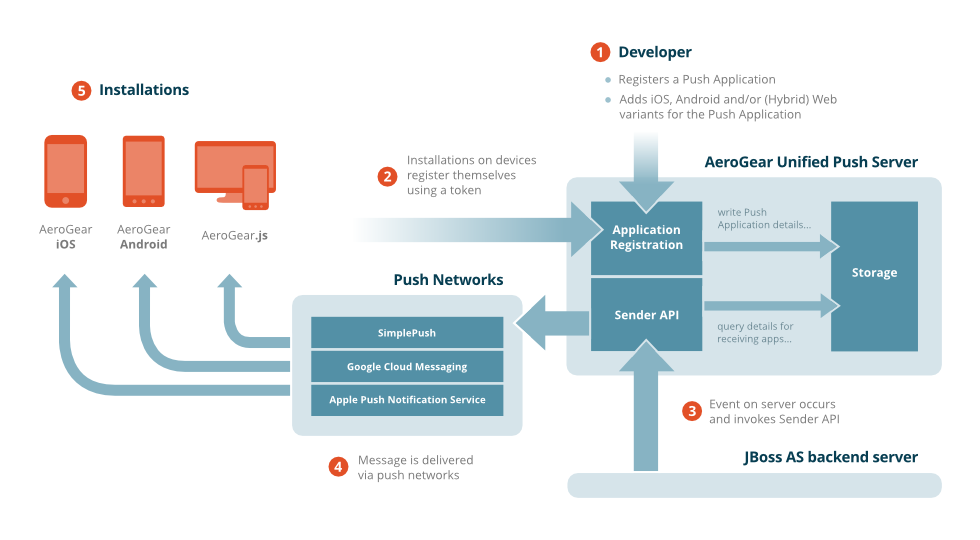
\includegraphics[scale=0.6]{img/aerogear_unified_push_server.png}
	\caption{\label{aerogear} Fonctionnement d'Aerogear}
\end{figure}


\begin{enumerate}
	\item L'administrateur doit commencer par créer une application Push, qui doit contenir au moins un Variant;
	\item Un appareil téléphonique demande un enregistrement en envoyant toutes les informations nécessaires à Aerogear (identifiant de l'appareil téléphonique, alias, etc). Ces informations sont stockées.
	\item Une requête est envoyée à Aerogear dans l'objectif d'envoyer une notification vers l'installation correspondant à un alias donné. Aerogear récupère toutes les informations nécessaires. La requête Push est ensuite traduite vers la plateforme correspondant au système d'exploitation correspondant à l'alias. La requête est ensuite envoyée vers la plateforme appropriée.
	\item La plateforme se charge de l'envoi de la notification vers l'installation correspondant à l'alias.
	\item L'installation reçoit la notification, et c'est à l'application téléphonique de gérer le traitement de cette notification.
\end{enumerate}

\subsection{Mise à jour d'Aerogear}

Mon premier objectif, au niveau d'Aerogear, était de mettre à jour le serveur Aerogear de Dynamease. Pour cela j'ai étudié la documentation officielle afin de connaître les différentes procédures de son installation.

Le serveur Aerogear se présente sous la forme d'une archive war. Une archive war, est une archive contenant tous les fichiers sources pour faire fonctionner une application serveur Java EE.

Le fonctionnement du service Aerogear nécessite un serveur Jboss et d'une base de données. Aerogear peut, théoriquement, fonctionner avec différentes bases de données relationnelles (H2, Mysql ou PostgreSQL). La base utilisée par Dynamease étant une base de données MySQL j'ai donc privilégié l'installation de la version correspondant à MySQL.

Plusieurs problèmes se sont accumulés lors de cette installation. En effet des erreurs étaient présentes durant le lancement du serveur. Après plusieurs recherches, il s'est avéré que le lien donné durant le processus d'installation pointé vers les sources d'une version non stable du projet. 

Après avoir récupéré un projet stable, j'ai dû faire face à une autre difficulté. Le serveur n'arrivait pas à utiliser la base de données MySQL. Après avoir effectué d'autres recherches il a s'est avéré que la version utilisée éprouvée quelques difficultés avec les bases de données MySQL et PostgreSQL, et que seules les bases de données du type H2 pouvait être gérées.

Les bases de données H2 fonctionnent sous l'environnement Java. Les données sont stockées sur un fichier unique. Afin d'y accéder de façon graphique, le logiciel officiel de cette base de données sera installé pour faciliter l'accès aux données s'y trouvant. Ainsi l'administrateur système pourra aisément réaliser ses requêtes de la même manière qu'il les aurait effectué sur une base de données MySQL.

Après son installation j'ai eu pour objectif de réaliser une image Docker d'Aerogear. L'explication de cette réalisation sera faite lors de la partie sur Docker.

\subsection{Mise à jour des notifications}

Après la mise à jour du serveur Aerogear j'ai également dû réaliser des mises à jour du côté des applications téléphoniques.

Pour les applications IOS, une mise à jour était nécessaire du fait que certaines méthodes utilisées pour l'enregistrement vers le serveur des notifications n'étaient pas rétrocompatible. Comme nous devions garder une version de l'application pour les personnes ayant encore une version IOS7 une vérification de la version de l'appareil est effectuée avant tout enregistrement au serveur. Il est probable que l'application Dynamease devienne, dans le futur, inaccessible pour les personnes possédant une version 7 d'IOS. En effet la version 8 permet beaucoup plus de liberté au niveau des notifications. Par exemple la possibilité d'ajouter des boutons d'action aux notifications pourrait être utilisée pour certaines fonctionnalités du service Dynamease.\\

Une autre mise à jour doit être effectuée sur la forme d'envoi des messages dans les notifications. L'ancienne version envoyée les informations sous la forme d'une chaîne de caractères préformatée pour l'affichage final. Ces chaînes de caractères étaient difficiles à traiter du fait que les informations pouvaient être dispersées. La solution la plus évidente à mettre en place était de faire passer des objets Json au travers les notifications. En effet, les objets Json sont très faciles à créer, à déchiffrer et de plus peuvent être écrits sous la forme d'une chaîne de caractères spéciaux.

Grâce à cette méthode il est plus facile d'effectuer un traitement sur les informations reçues et de déléguer à l'application téléphonique le tri des informations et l'affichage de celles-ci.

\section{L'environnement Docker}

\subsection{Fonctionnement de Docker}

Docker est un logiciel open source qui permet l'automatisation du déploiement d'application sur n'importe quel serveur ou machine Linux. Docker réuni une application et ses dépendances dans un container virtuel qui permet une portabilité plus aisée. En effet, la configuration nécessaire au fonctionnement d'une application sera déjà présente dans ce container. Ce container pourra être utilisé aussi bien sur une machine locale que sur un serveur, sans nécessiter de configuration sur la machine qui fera tourner l'application.

Docker propose également un serveur Hub dans le but de partager les différentes applications Docker réalisées par d'autres utilisateurs Docker.

Docker, contrairement aux machines virtuelles, n'a pas besoin de démarrer un système d'exploitation. Docker utilise directement le système d'exploitation de la machine sous-jacente. Docker exécute également ses processus de façon isolée.

Avant de continuer la présentation du travail effectué sur Docker, une définition, de quelques termes importants, doit être effectuée. 



\subsubsection{Container}

Le container est l’exécution d'une application. Chaque container détient une adresse IP privée et est exécuté sur un processus séparé.


\subsubsection{Images}

Une image Docker est la configuration d'une application au sein de Docker. Cette image peut être stockée sur le Hub de Docker afin que celle-ci soit partagée avec d'autres utilisateurs. Pour réaliser une image Docker, il faut rédiger un Dockerfile. Le Dockerfile représente le plan de fabrication de l'image Docker. Ce fichier doit contenir toutes les dépendances nécessaires au fonctionnement de l'application. Ce fichier peut être représenté comme un script qui est exécuté pour la création d'une image. Il faut réaliser ce script en prenant bien en compte qu'il s'agit de la configuration de l'environnement et non pas du lancement de l'application. Il est tout de fois possible de définir un script qui sera exécuté lors du démarrage du container.

Le Dockerfile doit aussi configurer les ports qui peuvent être ouverts sur le container. Par exemple pour un serveur Tomcat accessible depuis le port 8080, il faudra configurer l'image pour que le port 8080 du container soit accessible. À l'exécution du container, il est possible d'indiquer le port de la machine locale qui sera redirigé vers un des ports du container.

Cette image Docker nécessite d'avoir une image Docker de base. Par exemple pour réaliser l'image d'un serveur Jboss, nous avons besoin de Java, nous devrons donc partir d'une image Docker Java.


\subsubsection{Volume}

Un volume est un lien entre un répertoire se trouvant dans le container et un répertoire se trouvant sur la machine faisant tourner le container. Ainsi on peut utiliser des fichiers, se trouvant dans un dossier en local, dans le container. Le volume peut également être utilisé pour récupérer des fichiers se trouvant dans le container. Il est également possible de lier les volumes d'un container dans un autre container.

Les volumes sont à définir dans le Dockerfile en indiquant le répertorie du container qui contient les volumes. Les liens avec les répertoires en locale ou avec un autre container sont à définir lors de l'exécution du container.

\subsubsection{link}

Le \textit{link} est un lien entre deux containers. Comme nous l'avons vu précédemment, il est possible d'accéder à un port du container depuis un port de la machine locale. Il est également possible d'indiquer un lien entre deux containers docker pour que ceux-ci communiquent comme s'ils étaient sur deux serveurs différents. Le \textit{link} va renseigner dans le fichier host du container qui l'adresse IP de l'autre container à lier.

\subsection{Réalisation Docker pour le compte de Dynamease}

\subsubsection{Aerogear}

Comme nous l'avons vu précédemment, Aerogear nécessite d'un serveur JBOSS pour son fonctionnement. Nous allons donc partir d'une image JBOSS pour la réalisation de l'image Aerogear. L'accès à ce serveur se fera obligatoirement par le port 8080, car une vérification au niveau du service Aerogear est réalisée entre le port par lequel les requêtes entrent et le port par lequel l'application écoute.

Un volume sur les fichiers de base de données H2 sera également mis en place afin de pouvoir accéder à cette base de données, pour toutes importations, exportation ou modification de données.

\subsubsection{Nginx}

Nginx est un reverse proxy, qui permet de rediriger les requêtes entrantes sur un serveur vers un autre serveur distant, ou vers un autre port du même serveur.

Pour fonctionner Nginx ne nécessite que d'une distribution Linux. Debian est donc préféré aux autres distributions car c'est celle-ci qui est préféré pour tout serveur.

Le port d'accès par défaut à Nginx est 80. Ce port sera donc ouvert par le container, mais il est libre à l'utilisateur de ce container de redéfinir, lors du lancement du container, le port par lequel on accédera à ce container.

Un volume sera également créé vers le répertoire où sont stockés les fichiers de configuration Nginx, afin que la configuration Nginx, ne dépende pas d'une image mais d'un container.

\section{Démarrage automatique d'un environnement de travail}

\subsection{Fonctionnalités attendues}

Ce procédé doit permettre aux développeurs de Dynamease de pouvoir mettre en place de façon rapide et automatisée, un environnement de travail complet permettant l'accès aux différents services de Dynamease. 

Il doit également être possible de pré-remplir les bases de données Dynamease, avec des données, préexistantes, provenant de bases de tests ou bien de la base de production.

L'outil ainsi créé devra pouvoir être utilisé aussi bien sur des serveurs que sur les machines locales des développeurs. 

\subsection{Étude du cahier des charges}

Les environnements utilisés par Dynamease peuvent tourner grâce à des containers Docker. Pour l'outil qui sera développé, l'utilisation de ces containers sera mise en avant. Il sera donc nécessaire de déterminer l'ordre d'exécution de ces containers, en déterminant les différentes dépendances de ces containers.\\

Il faut également déterminer quelles sont les meilleures solutions pour la mise en place de l'intégration de données au démarrage de l'environnement Dynamease. L'environnement complet de Dynamease est constitué de plusieurs sous-environnements, les différents environnements nécessitant d'une intégration de données sont :

\begin{itemize}
	\item La base de données MySQL;
	\item La base de données Ldap;
	\item La base de données liée à Aerogear;
	\item Les fichiers de configuration du serveur Dynamease.
\end{itemize}

Il faudra donc déterminer, pour chacun de ces environnements, quels sont les techniques permettant une intégration de données.

De plus il doit être possible de démarrer un environnement vide. il faudra donc gérer ce cas de figure, en initialisant les bases de données de manière à ce qu'elles soient utilisables par l'environnement complet de Dynamease.

\subsection{Réalisation de l'outil}

\subsubsection{Détermination des dépendances}

\begin{figure}[!h]
	\centering
	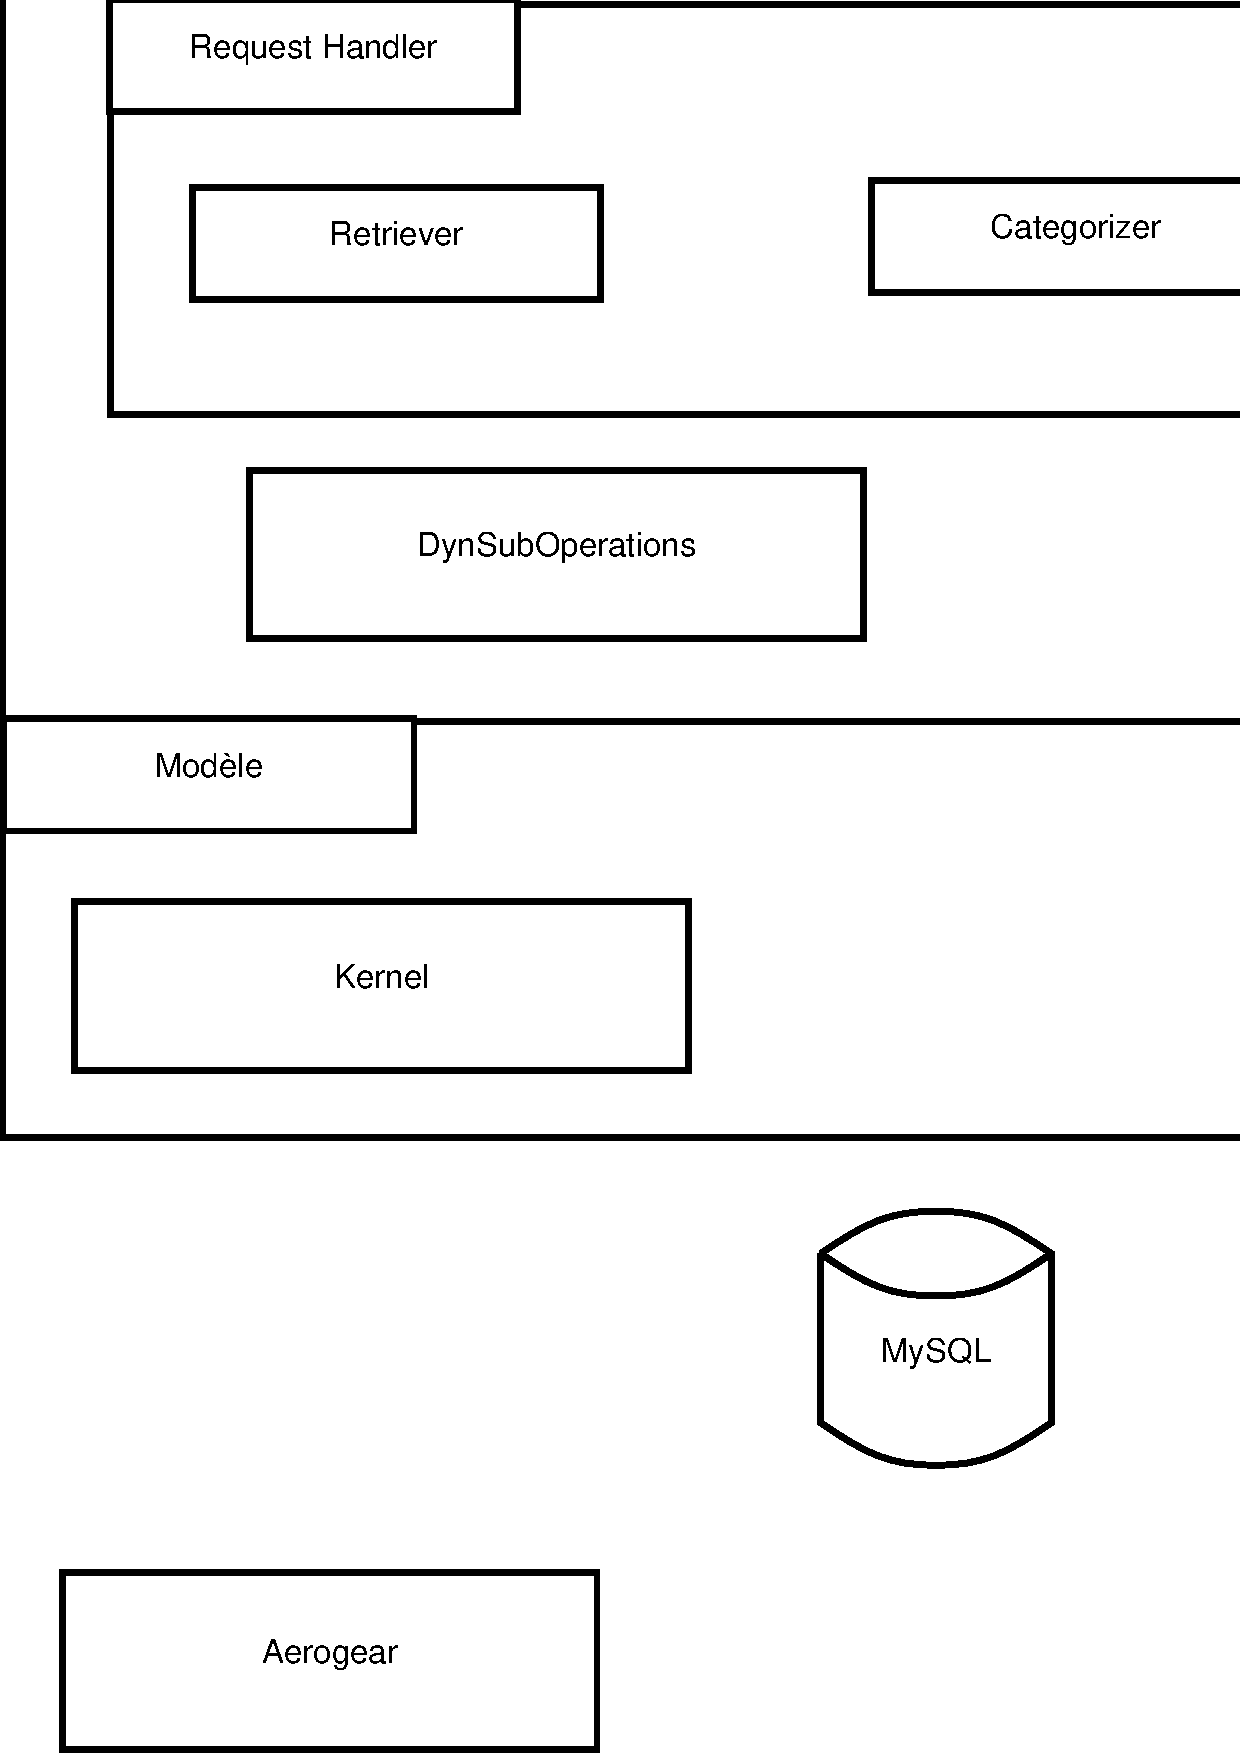
\includegraphics[scale=0.4]{img/pyramide.pdf}
	\caption{\label{pyramide} Pyramide des dépendances de l'environnement Dynamease}
\end{figure}

Nous allons étudier le diagramme ci-dessus, de manière descendante. Tout en haut nous avons l'environnement Nginx, celui-ci nécessite la mise en place des environnements Tomcat et Aerogear pour fonctionner correctement. L'environnement Tomcat nécessite l'existence des bases de données MySQL et Ldap. 

Donc il nous faudra lancer l'environnement l'ordre suivant :

\begin{enumerate}
	\item La base de données MySQL;
	\item La base de données Ldap;
	\item Aerogear;
	\item Tomcat;
	\item Nginx.
\end{enumerate}

\subsubsection{Récupération et utilisation des données}

Le fonctionnement de l'environnement Dynamease dépend de plusieurs données. On peut séparer les données à récupérer en deux catégories, les données de configuration et les données de stockage d'informations.

Les données récupérées, par le serveur Tomcat de Dynamease, sont essentiellement des données de configuration. Cette configuration permet à Dynamease de connaître les adresses internet des différents services nécessaires à son fonctionnement. Ces adresses peuvent être différentes d'un environnement à un autre selon l'emplacement de démarrage de l'application Dynamease. Le mieux est donc d'avoir ces fichiers stockés sur l'emplacement de démarrage de l'environnement.

Pour ce type de donnée, il sera demandé la création d'une variable d'environnement par l'utilisateur afin de lui permettre de préciser à l'outil, l'emplacement des différents fichiers de configuration de Dynamease.

Des fichiers de configuration par défaut seront présents dans l'outil. Si l'utilisateur ne désigne pas de répertoire contenant ces fichiers de configuration, un message sera affiché pour le prévenir que des fichiers de configuration par défaut seront utilisés, mais que cela peut entraîner quelques dysfonctionnements.\\

En ce qui concerne les données des différentes bases de données, celles-ci peuvent être stockées indépendamment de leurs bases de données d'origine. Seul leur intégration sera différente.

Il nous reste donc trois bases de données à remplir avec nos fichiers de données. Leurs techniques d'intégration étant différentes nous allons les étudier pour chaque base de données. 

Deux solutions de stockage peuvent être étudiées, on pourrait utiliser les volumes de chaque container, en intégrant les données. Cette méthode risque d'être assez limitée sachant que chaque utilisateur devra disposer des fichiers de données afin de les intégrer dans son environnement. La seconde solution serait d'utiliser une nouvelle image Docker qui aura pour rôle le stockage de tous les fichiers de données. Cette solution permettrait de pouvoir utiliser n'importe quelle base de données sans récupérer les fichiers de données. C'est cette seconde solution que nous allons développer par la suite.

Cette solution prend en compte que le container de données contient des volumes pour stocker les fichiers de données. Or, comme nous l'avons vu précédemment, les volumes créés des liens symboliques depuis les volumes du container vers les répertoires situés sur la machine faisant tourner le container. Donc le container serait opérationnel uniquement sur la machine l'ayant créé, si ce container se trouve sur un autre système, il se peut que les liens ne pointent sur aucun fichier ou sur de mauvais fichiers.

On a également vu qu'on pouvait exécuter des commandes lors de la création du container. L'idée est d'utiliser un script de démarrage du container, qui nous servira à déplacer et trier les fichiers de données vers de nouveaux répertoires.

Grâce à cette récupération nous pouvons maintenant faire un traitement pour chaque fichier selon le type de base de données où celui-ci doit être inclus.\\

Il est aussi prévu de permettre aux utilisateurs de cet outil de lancer un environnement de travail, vide. C'est-à-dire seulement avec les bases de données initialisées, mais sans données. Pour cela l'image docker de stockage des données sera généré avec les fichiers d'initialisation de chacune des bases de données. Un script de démarrage aura pour rôle de déterminer si des fichiers d'intégration de données sont présents, si c'est le cas, ces fichiers seront déplacés vers le répertoire correspondant à la base de données, sinon ce seront les fichiers d'initialisation qui y seront placés. 

\begin{figure}[!h]
	\centering
	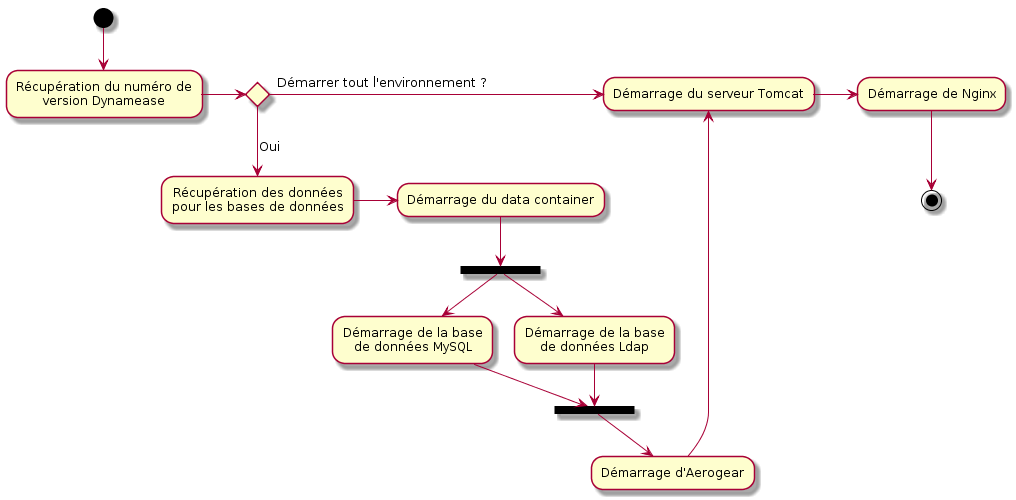
\includegraphics[scale=0.5]{img/activity_outil.png}
	\caption{\label{activity_outil} {Résumé du fonctionnement de l'outil}}
\end{figure}
\subsubsection{Récupération de la version Dynamease}

Le lancement de l'environnement de travail Dynamease, doit inclure un numéro de version du serveur Dynamease. 

Chaque version de Dynamease est présente sur le \textit{repository} Docker de Dynamease. Chaque nouvelle version déposée sur le serveur Git est récupérée par le serveur Jenkins. Celui-ci aura pour charge de vérifier le bon fonctionnement de la version déposée. Si celle-ci est correcte alors une nouvelle image Docker du serveur est créée avec le nom du commit comme numéro de version.

La création d'une image docker Dynamease, nécessite d'abord la compilation de l'ensemble du code source de Dynamease, de la récupération des archives (war) du serveur et enfin de leur intégration vers la nouvelle image Docker.

Le script de démarrage de l'environnement prendra en paramètre un numéro de version. Il vérifiera alors si l'image est présente en local, si ce n'est pas le cas l'image sera téléchargée depuis le serveur Docker, si elle existe sur le serveur distant. Si elle n'existe pas sur le serveur distant un message d'erreur est renvoyé.

Grâce à cette méthode, il est possible de démarrer rapidement n'importe quelle version de Dynamease, car l'image est forcément déjà créée.

\section{Amélioration des applications téléphoniques}

Nous allons maintenant aborder les différentes améliorations que nous devions réaliser après la réalisation de plusieurs tests de performance.

\subsection{Récupération des contacts Ios}

En début de stage un problème nous a été reporté par un utilisateur de l'application Iphone. L'application ne démarrait pas sur son Iphone. Juste après la connexion de l'utilisateur, l'application ferme subitement. Nous avons donc tenté de reproduire ce dysfonctionnement sur nos téléphones de test. Il nous était impossible de déterminer d'où venait l'erreur.

Nous avons donc demandé le modèle d'Iphone et la version IOS afin de pouvoir reproduire la procédure d'erreur dans les mêmes conditions. Mais encore une fois l'application semblait très bien fonctionner sur nos téléphones de test. Nous avons également demandé à l'utilisateur de se connecter à l'aide d'un de nos téléphones de test, mais l'erreur ne s'est pas reproduite.

Nous en avons donc conclu que l'erreur devait provenir d'une configuration spéciale de l'Iphone de l'utilisateur.

Nous avons listé les différentes méthodes exécutées par l'application au démarrage, afin de déterminer celles qui auraient pu interagir directement avec une configuration spéciale de l'utilisateur.

\begin{figure}[!h]
	\centering
	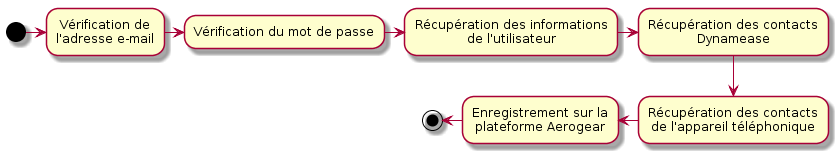
\includegraphics[scale=0.5]{img/activity_ios.png}
	\caption{\label{activity_ios} {Parcours de la connexion utilisateur}}
\end{figure}

Les différentes méthodes exécutées par l'application étaient, la récupération des informations de l'utilisateur auprès du serveur Dynamease, la récupération des contacts du portable et l'inscription sur le serveur Aerogear.

Après une observation sur les logs des serveurs Dynamease et Aerogear, nous nous sommes aperçus que les données de l'utilisateur étaient bien envoyées mais que le serveur Aerogear ne recevait pas de requêtes d'inscription.

L'erreur provenait donc de la récupération des contacts. De plus nous avons remarqué que l'utilisateur avait énormément de contact. Le problème pouvait donc provenir soit d'un contact particulier de l'utilisateur dont les informations étaient mal traitées, ou bien que le nombre important de contacts faisait fermer subitement l'application.

Pour éviter de demander la liste de contacts de l'utilisateur nous avons décidé en premier lieu de se pencher sur la seconde solution en créant des centaines de contacts que nous importerions par la suite dans le téléphone de test. L'application arriva parfaitement à traiter ces centaines de contacts.

Nous avons donc dû demander la liste de contacts de l'utilisateur dans le but de détecter quel était le contact qui produisait cette erreur, et qu'elle était la cause.

Après l'importation de cette liste de contacts, nous avons remarqué que l'erreur se produisait également sur les téléphones de tests. Après une observation des logs générés par l'application il est apparu qu'il existait un contact dont le nom commencé par le caractère $'@'$.

Les contacts dans l'application Iphone sont stockés dans un dictionnaire (ensemble clefs valeurs). Les clefs sont représentées par le nom de l'utilisateur et les valeurs sont les informations relatives à l'utilisateur. La clef est donc de type chaîne de caractère. Or en Objective-C le caractère $'@'$ est un caractère spécial. L'Iphone n'arrivant pas à interpréter ce caractère l'application ferme subitement.

Afin de régler ce type de problème, un caractère spécial $'\textbackslash'$ est ajouté devant chaque caractère spécial pouvant être trouvé dans le nom ou les informations de l'utilisateur. Ce caractère a pour fonction, dans l'Objective-C de signifier à l'application de ne pas interpréter le caractère spécial qui le suit. 

\subsection{Recherche et récupération automatique des contacts}


\subsubsection{Recherche de contact}

\begin{figure}[!h]
	\centering
	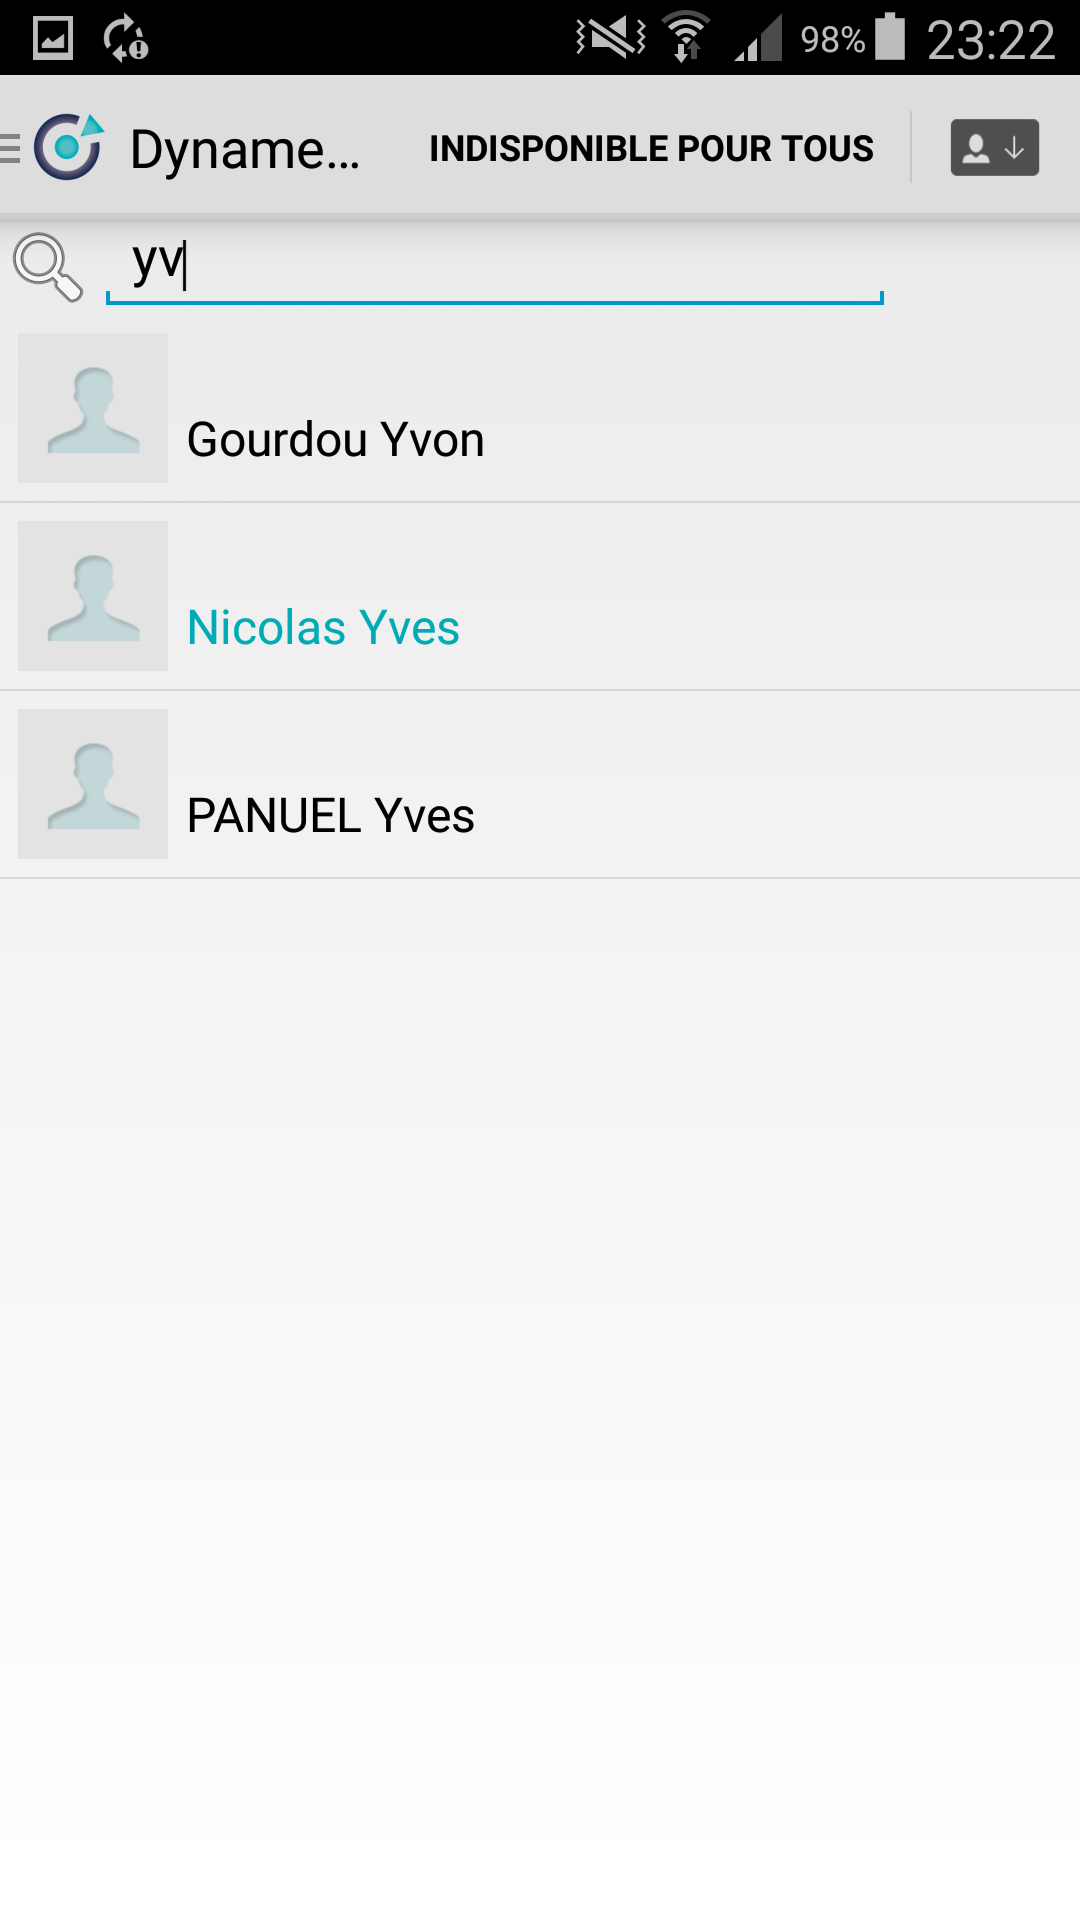
\includegraphics[scale=0.1]{img/recherche.png}
	\caption{\label{recherche} {Vue de la recherche dans la liste de contacts sur l'application Android}}
\end{figure}

L'application Téléphonique Android, permet aux utilisateurs d'avoir une liste de contact. Cette liste de contact est triée par défaut dans l'ordre alphabétique par rapport aux noms de famille des contacts. De plus une barre de recherche est disponible pour faire une recherche dans cette liste.

La version précédant ma correction, n'effectuait la recherche uniquement sur le nom, de plus sur de longues listes de contact, la recherche pouvait prendre beaucoup de temps.

La première étape pour effectuer une correction est d'observer la technique utilisée pour cette recherche.\\\\

En premier lieu, j'ai étudié les différents moyens de stockage que proposait Android. Il propose trois moyens de stockage qui sont :

\begin{enumerate}
	\item Stockage par le biais de clefs/valeurs;
	\item Stockage dans un fichier texte;
	\item Stockage à l'aide d'une base de données SQL Lite.
\end{enumerate}

La première technique peut être utilisée pour de petites valeurs à usage récurrent, comme le nom de l'utilisateur, son numéro de téléphone, etc.

Le fichier texte est surtout utilisé si on doit générer des fichiers de données, pouvant être récupéré par l'utilisateur.

La base de données SQL est utilisée pour stocker des listes de données suivant le même schéma.

C'est cette dernière option qui nous intéresse pour le stockage de la liste de contact. C'est effectivement cette technique de stockage qui est utilisée pour le stockage des contacts.

Un contact normal est représenté par son nom, son prénom, son numéro de téléphone. Un contact Dynamease est représenté par son nom, son prénom et son identifiant Dynamease. C'est deux types de contact sont stockés dans la même table de données, et sont différenciés par une variable booléenne qui est à vrai si le contact est un contact Dynamease et est à faux sinon.\\\\

L'algorithme anciennement utilisé pour la recherche des contacts suivait le diagramme suivant :

\begin{figure}[!h]
	\centering
	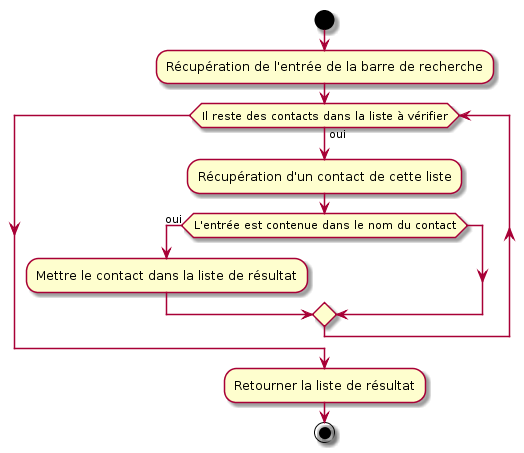
\includegraphics[scale=0.8]{img/activity_retrieve_old.png}
	\caption{\label{activity_retrieve_old} {Diagramme d'activité de l'algorithme anciennement utilisé pour la recherche des contacts}}
\end{figure}

Chaque fois que l'utilisateur entre une lettre dans la barre de recherche, le processus de la recherche est lancé. Pour chaque contact de la liste, on vérifie si l'ensemble des lettres entrées dans la barre de recherche, est présent dans le nom du contact. Si on trouve une correspondance entre l'ensemble des lettres et le nom du contact on ajoute ce contact à la liste de retour. Et on effectue cette correspondance pour chaque contact.

Ce processus est long en raison la recherche sur toute la liste de contact à chaque ajout de lettre dans la barre de recherche. L'autre problème flagrant est que la recherche n'est effectuée que sur le nom.

\newpage

La première résolution de ce problème suit le processus suivant :

\begin{figure}[!h]
	\centering
	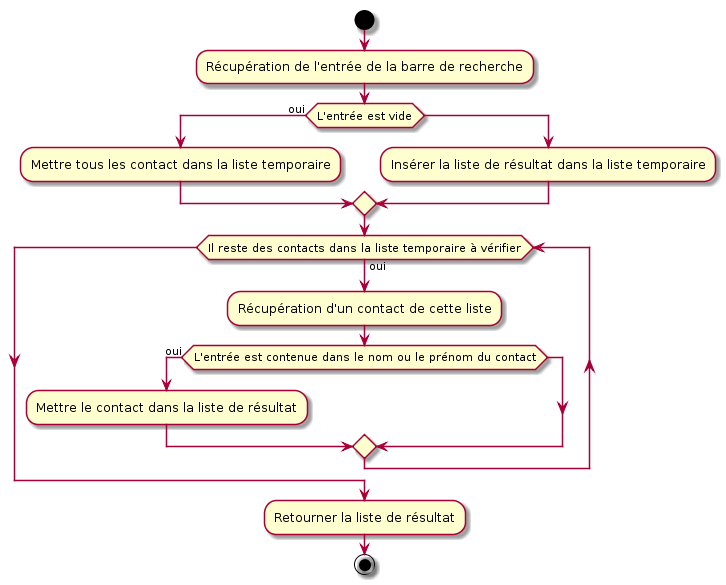
\includegraphics[scale=0.6]{img/activity_retrieve_new.png}
	\caption{\label{activity_retrieve_new} {Diagramme d'activité de l'algorithme utilisé pour la recherche des contacts}}
\end{figure}

Avant toute recherche la liste de contact est contenue dans le résultat à retourner. Par défaut tous les contacts correspondent à une recherche vide. À chaque ajout de lettre, on recherche dans la liste dernièrement retournée les contacts ayant l'ensemble des lettres de recherche dans leur prénom ou dans leur nom. Si une correspondance est trouvée alors le contact est ajouté dans une liste temporaire. Une fois tous les contacts vérifiés, on remplace la liste de résultat par la liste temporaire, et on renvoie la liste de résultat. Et on continue sur le même principe à chaque ajout de lettre

\newpage

Le problème de cette solution c'est que l'ordre des mots de recherche est important faire une recherche $"\textit{nom prénom}"$ ne sera pas interprété de la même façon que la recherche $"\textit{prénom nom}"$.

\begin{figure}[!h]
	\centering
	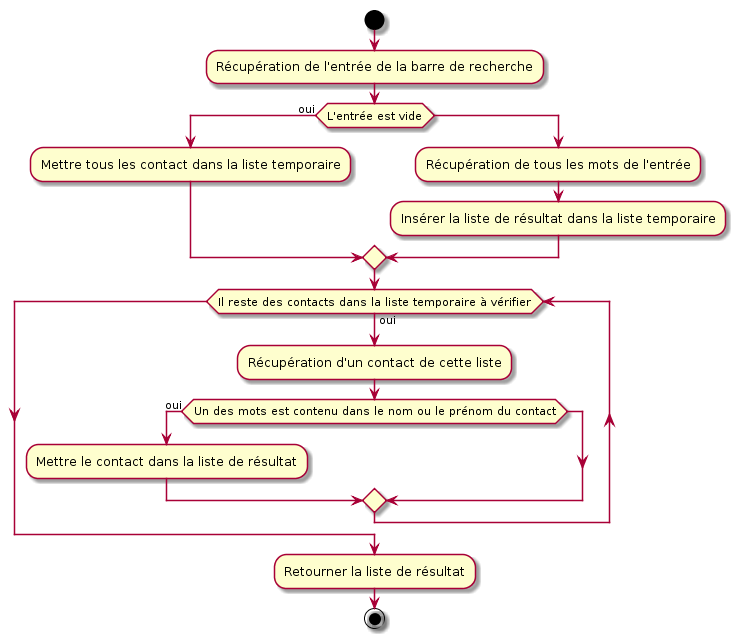
\includegraphics[scale=0.6]{img/activity_retrieve_better.png}
	\caption{\label{activity_retrieve_better} {Amélioration du diagramme d'activité de l'algorithme anciennement utilisé pour la recherche des contacts}}
\end{figure}

On reprend le même principe que précédemment, mais cette fois-ci on fait un travail supplémentaire entre l'ajout d'une lettre et la recherche dans la liste de contact. On sépare les différents mots de la barre de recherche. On estime qu'il y a un nouveau mot à chaque fois que la barre espace est pressée. On sépare donc les différents mots, et on les stocke dans un tableau. Ensuite la recherche dans les contacts doit correspondre à chaque mot se trouvant dans le tableau. Si un mot ne trouve aucune correspondance, ni dans le nom, ni dans le prénom, alors le contact ne sera pas ajouté à la liste de résultat. Tous les mots doivent correspondre au nom ou au prénom, pour que le contact soit ajouté dans la liste de résultat.

\newpage

\subsubsection{Récupération des contacts du téléphone}

\begin{figure}[!h]
	\centering
	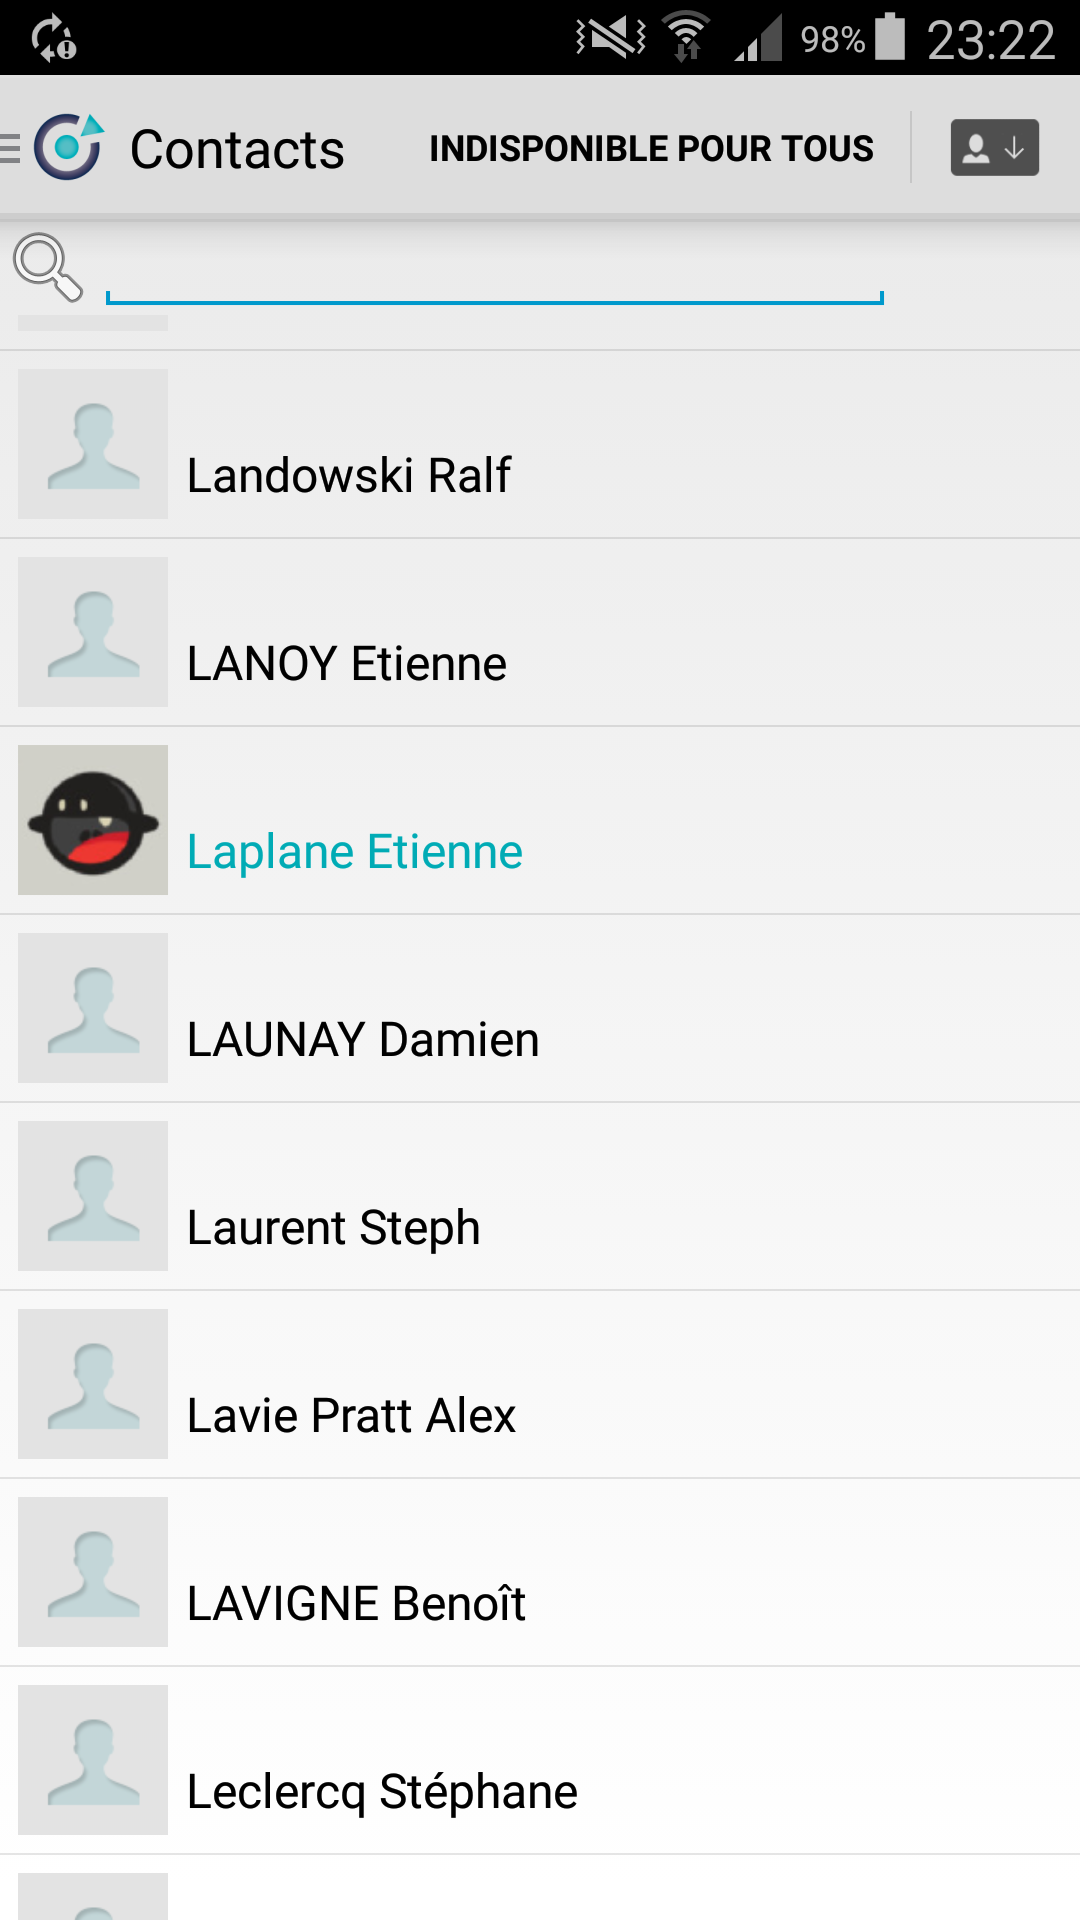
\includegraphics[scale=0.1]{img/contact.png}
	\caption{\label{contact} {Vue de la liste de contacts sur l'application Android}}
\end{figure}

La récupération des contacts ne semblait s'effectuer qu'une seule fois, lors du premier lancement de l'application. De plus il existait quelques problèmes au niveau du temps de récupération des contacts. Plus la liste de contact était grande et plus le temps de récupération était long (par exemple pour une liste de contact de 10000 contacts le chargement pouvait être de quelques jours).\\

Après une inspection du code, j'ai pu remarquer que, l'activité de la liste de contact se chargeait de la récupération des contacts à chacun de ses lancements. Or cette récupération avait une mauvaise condition pour la récupération des contacts.

La liste de contact est triée par ordre alphabétique dans la base de données de Dynamease, c'est également le cas pour la liste de contact du téléphone. L'activité vérifie que le nombre de contacts dans la liste de contact du téléphone est égal au nombre de contacts de la liste de contact de l'application Dynamease. Si ce n'est pas le cas une vérification est effectuée. Le problème se situe sur la suite du procédé. Le \textit{cursor} permettant la récupération est programmé pour récupérer les contacts en partant de l'index correspondant au nombre de contacts dans la liste de contact Dynamease moins un. Or les contacts stockés dans la base de données du téléphone ne sont pas triés par ordre chronologique mais par ordre alphabétique. Donc si un contact, après le premier démarrage, est ajouté au début de la liste de contact du téléphone, alors il ne sera jamais récupéré par l'application, et le programme fera une récupération de contact à chaque démarrage de l'activité.

La recherche est maintenant effectuée sur l'ensemble de la liste de contact du téléphone et une vérification sur l'existence des contacts est également effectuée, afin de ne pas avoir de doublon.\\

La récupération des contacts s'effectue par des \textit{Task}. Comme un \textit{Thread}, plusieurs \textit{Task} peuvent être en fonction "simultanément". Donc à chaque fois que l'activité de la liste de contact est lancée, la \textit{Task} de récupération des contacts est lancée. Donc le temps processeur est divisé entre ces deux \textit{Task}.

Pour améliorer cette récupération une condition est rajoutée pour déterminer si une récupération est déjà en cours afin de ne pas rediviser le temps processeur. De plus un bouton d'actualisation de la liste de contact a été ajouté. Dorénavant, la récupération des contacts s'effectue seulement si la liste de contact de l'application Dynamease est vide ou si l'utilisateur appuie sur le bouton d'actualisation.

\subsubsection{Récupération des images de profil}

Chaque utilisateur Dynamease peut avoir une image de profil. Cette image de profil est affichée sur la liste de contact, de tous les utilisateurs Dynamease ayant reçu une carte de visite de l'utilisateur propriétaire de l'image.

Il est apparu également qu'à chaque affichage de la liste de contact, dans l'application Android, une requête pour récupérer les images de profil Dynamease est envoyée. Ces requêtes n'ont pas forcément lieu d'être effectuées à chaque affichage. En effet, le changement d'image de profil est beaucoup trop rare pour qu'une requête soit envoyée aussi couramment.

La requête de récupération des images s'effectue grâce à une requête Json. Le résultat de la requête se présente sous la forme d'une suite de caractères représentant l'image. Cette récupération est effectuée pour l'affichage des images dans la liste de contact. Il faut donc trouver une solution pour ne pas avoir à effectuer une requête pour l'affichage des images.

Le plus simple est de stocker les images sur l'appareil de l'utilisateur. Nous avons exploré précédemment les différentes techniques de stockages qu'offrait Android. La meilleure solution est d'utiliser l'écriture de fichier. Ce type de stockage, effectue, par défaut, la sauvegarde dans un dossier spécifique à l'application et qui ne peut être accédé que par celle-ci. On récupérera donc la suite de caractères pour la stocker dans un fichier.

La récupération des images doit au moins être effectuée une fois. Pour cela on suivra l'algorithme suivant :

\begin{figure}[!h]
	\centering
	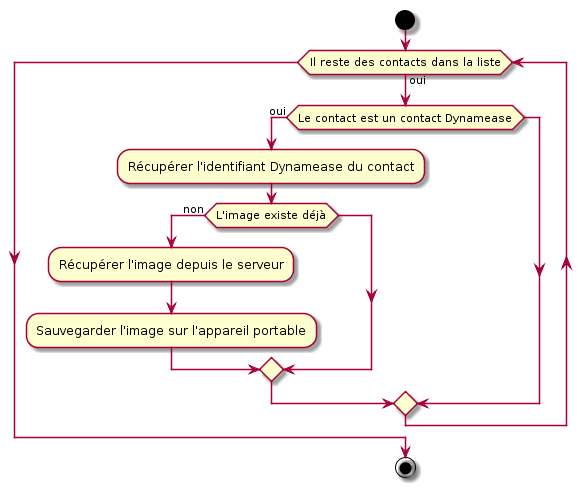
\includegraphics[scale=0.5]{img/activity_image.png}
	\caption{\label{activity_image} {Diagramme d'activité pour la récupération d'image de profil}}
\end{figure}

Lors de l'affichage de la liste de contact, à chaque contact Dynamease on fait la vérification suivante. On vérifie si l'image de profil est présente dans le répertoire de l'application Dynamease. Si l'image n'est pas présente, on envoie une requête vers le serveur Dynamease, afin de la récupérer. Une fois cette image récupérée, on stocke la suite de caractères récupérée dans un fichier. Le fichier de sortie sera nommé comme l'identifiant Dynamease du contact. si le contact ne dispose pas d'image de profil alors ce sera l'image par défaut qui sera écrite dans le fichier de sortie.

Ainsi l'affichage des images se fera par le biais de la récupération des fichiers images présents sur l'appareil téléphonique.

\subsubsection{Améliorations possibles}

La récupération des images ne se fait qu'une seule fois. Or il est possible qu'un contact change son image de profil. Aucune mise à jour ne sera effectuée avec la méthode actuelle. Il faut donc penser à une solution pour que les images de profil soient mises à jour. Pour cela on pourrait utiliser le bouton de rafraîchissement de contact déjà utilisé pour mettre la liste des contacts du téléphone à jour.

Il est aussi possible de créer une nouvelle requête permettant de vérifier si une image de profil a récemment été mise à jour. L'application téléphonique enverrait la date à laquelle l'image de profil fût créée. Si la date reçue est antérieure à la date de mise à jour de l'image de profil, celle-ci serait renvoyée.


\section{Amélioration continue du service par la mise en place d'outils}

La mise en place d'outils d'aide à la mesure des performances est importante pour les entreprises afin de leur permettre d'affirmer le bon fonctionnement de leurs produits. Dynamease ne disposait d'aucun outil pour la réalisation de tests de performance. Chacun d'entre eux était fait manuellement.

Afin de mettre en place ces outils il m'a fallu d'abord faire la liste des différents outils dont j'aurais besoin. Une fois cette liste récupérée je devrais alors déterminer les fonctionnalités de chacun des outils qui seront indispensables pour Dynamease. À la suite de quoi je devrais rechercher les outils proposant les fonctionnalités recherchées.

La mise en place de ces outils nécessitera un travail en amont dans le but de déterminer les métriques à utiliser et également déterminer quelles sont les limites acceptables pour Dynamease.\\

La liste des différents tests de performance, qui devraient être effectuées à Dynamease, est la suivante :

\begin{itemize}
	\item Tests d'intégration web;
	\item Tests d'intégration des applications téléphoniques;
	\item Tests de performance des serveurs;
	\item Supervision applicative des éléments.
\end{itemize}

\subsection{Test d'intégration web}

Le but de cette partie est de vérifier le bon fonctionnement du serveur Dynamease lors de l'appel des différentes requêtes. Aussi bien celles appelées par l'application web que celles appelées par les applications téléphoniques.

Il est nécessaire que l'outil utilisé puisse générer un fichier unique de tests. De plus il doit être possible de lancer ces tests automatiquement. L'outil doit être capable aussi bien d'envoyer des requêtes REST que des requêtes JsonRPC.

Après plusieurs recherches, l'outil SOAPUI fût choisi. Malgré son nom, cet outil permet d'envoyer des requêtes REST et RPC. De plus la configuration des tests d'intégration est stockée dans un fichier XML, et donne la possibilité de lancer tous les tests via Maven. Ce qui est très utile sachant que l'archive du serveur Dynamease est construite grâce à Maven

\subsection{Tests d'intégration des applications téléphoniques}

Ces tests permettent d'effectuer des parcours d'utilisateurs sur les applications téléphoniques. Ces tests permettent de savoir si les applications sont fonctionnelles. Ils peuvent également être utilisés pour tester l'interface des applications. Le service Dynamease étant présent sur Iphone et Android, il serait intéressant d'avoir un outil nous permettant d'avoir la possibilité d'effectuer ces tests sur ces deux plateformes. 

Nos applications sont développées de façon parallèle et non pas par l'intermédiaire d'un \textit{framework} permettant de réaliser une application sur les deux systèmes d'exploitation, Android et Iphone. 

L'application Dynamease utilise des méthodes de bas niveau sur les deux systèmes. De plus certaines méthodes sont présentes sur un des systèmes mais pas sur l'autre. Il est donc difficile de générer deux applications à partir d'un même code source. L'utilisation d'un tel \textit{framework} est donc impossible pour une telle application.

Bien que les applications aient quelques différences et ne puissent pas être testées par une seule configuration de tests, il est tout de même intéressant d'utiliser un seul outil pour ces tests. Un seul outil permettrait de faire qu'une seule formation. Certaines parties de ces deux applications sont identiques il est donc envisageable d'utiliser quelques parties d'une configuration d'une application pour l'autre configuration.

Après quelques recherches j'ai pu trouver les outils tels que Appium et MonkeyTalk. Après une étude des documentations de chacun de ces outils, il est apparu que MonkeyTalk proposait plus de fonctionnalité et une meilleure documentation. Ce qui faciliterait son apprentissage et donc sa mise en place.


\subsection{Ce qu'il reste à faire}

Je dois encore faire un travail de recherche pour les tests de performance des serveurs et de l'interface web. Bien que quelques outils soient quand même listés, il faut encore tester chacun de ces outils afin de déterminer lequel de ces outils et le plus à même de répondre à nos attentes.

Je dois également mettre en place l'outil MonkeyTalk pour les tests d'intégration des applications téléphoniques.

Une recherche sur les différentes fonctionnalités que proposeraient les outils de supervision est également à prévoir. 